\chapter{Results and Discussion}
TODO da rivedere se coerente

In questa sezione sono presentati, i risultati del migliore approccio, descritto anche nel Capitolo METODOLOGIA vari tentativi fatti, quelli del processo di raffinamento risultati ottenuti conclusions are drawn regarding the study of OoM and the improved visualization of skeletal clusters.
The original planned work underwent modifications due to the limitations of a reduced and unbalanced dataset, coupled with challenges in finding additional complete and consistent samples to enrich the dataset.
Although it was not always easy, addressing and resolving the issues inherent in this type of research proved to be immensely enriching both personally and professionally.
It posed a challenge and provided a glimpse into what we might have to confront in the future, and we are grateful for the opportunity to have had this experience.

In the following section, a synthesis of the results achieved and potential outcomes is presented.
It particularly focuses on performance analysis in terms of operating conditions and further future developments aimed at improving the obtained results.

\section{Graph-based Framework}
The OoM was classified using three distinct features: velocity, acceleration and angular momentum, as described in Section \ref{subsec:alg_features}.
For each feature, we applied two different similarity functions, as part of the pipeline explained in Chapter \ref{sec:graph_method}.
The two similarity functions are the \textit{Cosine Similarity} (concept explained in Section \ref{subsec:cosine_sim}) and a custom function described in Section \ref{sec:starting_point}.

In Table \ref{tab:clust_results} we can see that the Cosine similarity outperforms the custom-made function. 
Therefore, it was chosen as the similarity function for this specific dataset.

\begin{table}[H]
  \centering
  \begin{tabular}{||>{\centering\arraybackslash}p{4.3cm}||>{\centering\arraybackslash}p{2.0cm}||>{\centering\arraybackslash}p{2.7cm}||>{\centering\arraybackslash}p{4.4cm}||}
  \hline
  \textbf{Similarity Function} & \textbf{Speed} & \textbf{Acceleration} & \textbf{Angular Momentum} \\
  \hline
  Cosine & 28.3\%  & 26.7\%  & 36.6\%  \\
  \hline
  Custom & 18\%  & 21.1\%  & 34.2\%  \\
  \hline
  \end{tabular}
  \caption{Classification accuracy over the whole dataset obtained by using the two different similarity functions}
  \label{tab:clust_results}
\end{table}

From here on, the graphs will reflect the results obtained using cosine similarity as the measurement method.
While these results may not be exceptional, they still outperform a random approach, in which two random nodes are selected and compared to the ground truth. \\
Infact such an approach, achieves an accuracy of 19\% 
The formula to calculate the probability of picking at least one joint of the two is shown in Equation \ref{eq:prob_rand}
\begin{equation}
  \mathbb{P}(\textit{"picking at least one of the two joints"}) = 2 \cdot \frac{2}{20} \cdot \frac{18}{20} + \frac{2}{20} \cdot \frac{2}{20} = \frac{19}{100}
  \label{eq:prob_rand}
\end{equation}
TODO controllare probabilità

In Figure \ref{fig:wdc_results} we can see the distribution of the results for each edge of the dataset with respecto to their ground truth.
\begin{figure}[H]
  \centering
  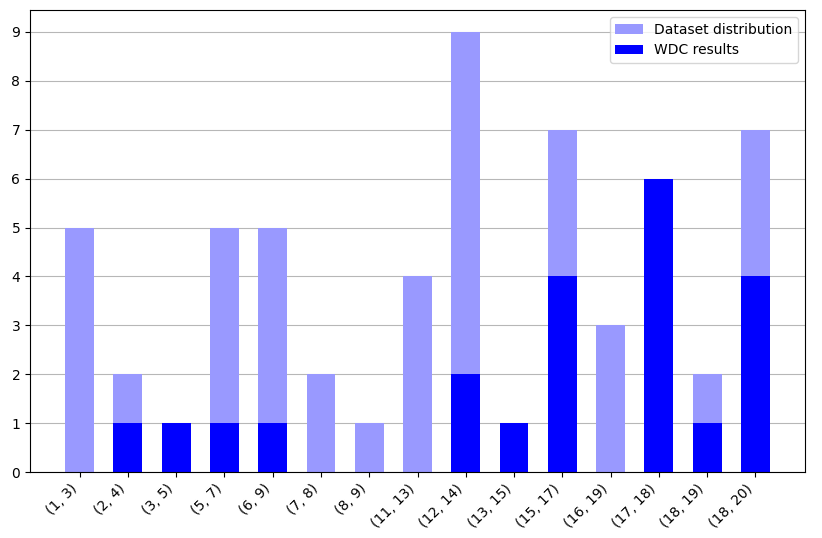
\includegraphics[width=0.85\textwidth]{wdc_results.png}
  \caption{Joints and frequency of the dataset and the correctly classified WDC algorithm}
  \label{fig:wdc_results}
\end{figure}
TODO rifare




\clearpage

\section{Clusters Stabilization}
In this first example, in Figure \ref{fig:stabilization_results}, we can observe the results of stabilization of three clusters with the same color scheme applied on two different time instants. 
In (a), the preceding time instant is visible, while (b) showcases the subsequent time instant in an unstabilized state. 
In (c) instead, the subsequent time instant with clusters stabilized.
\begin{figure}[H]
  \centering
  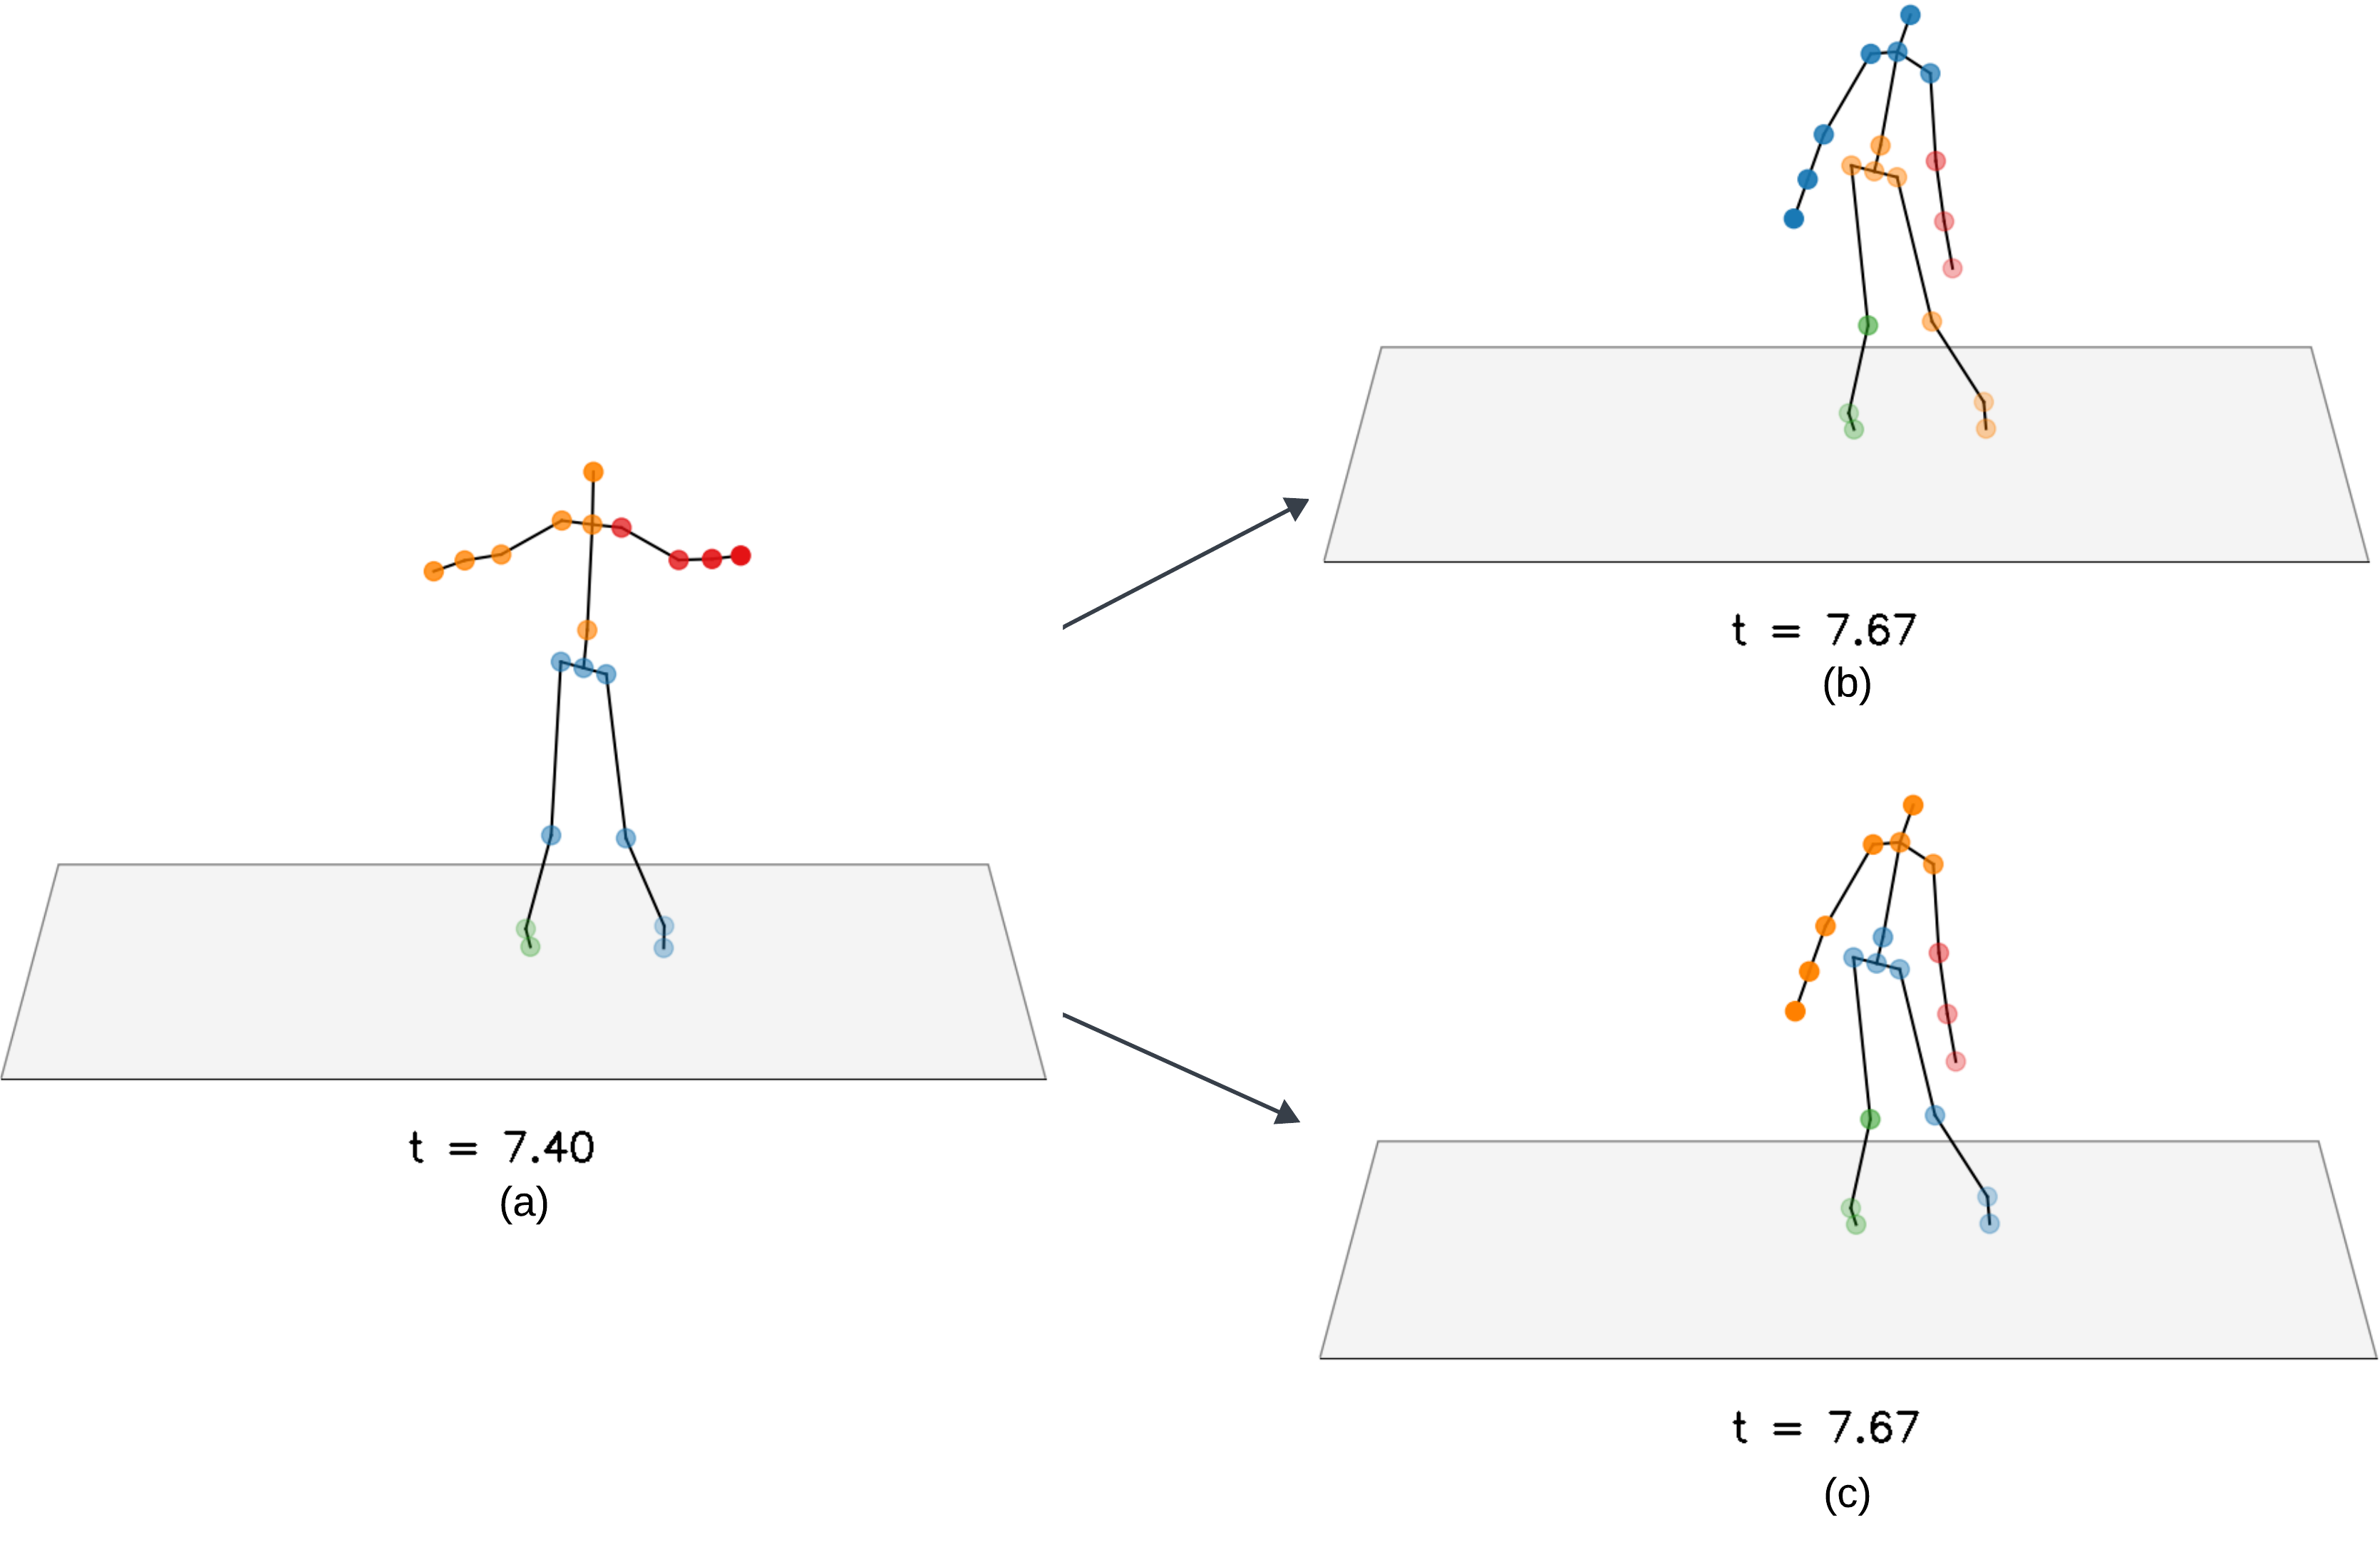
\includegraphics[width=0.9\textwidth]{ClustersStabilization.png}
  \caption{Clustering at $t=7.40$ (a), $t=7.67$ unstabilized (b), and $t=7.67$ stabilized (c).}
  \label{fig:stabilization_results}
\end{figure}

A further extension of this concept for visualization purposes can be applied by analyzing a movement evolving in realtime, by recording a small segment of video, which is able to provide a better view of the stabilization outcomes.
The transition smoothing algorithm explained in Section \ref{subsec:clusters_smoothing} is here visualized in the videos whose link has been embedded in the QR code in Figure \ref{fig:qr_movements}. \\

These 3 QR codes lead to a video that represents the same movement in the 20 joints skeleton, where the dancer begins from a stance with slightly spread legs and the left arm raised upwards.
Throughout the movement, the left arm descends while moving backward, the torso leans forward, taking the right arm along with it, and the left foot lifts off the ground, walking back to follow the left arm.\\

The first QR (Figure \ref{fig:qr_movement_pure}) leads to the original clustering method without the application of any stabilization method, visually it can be clearly seen how the instability of the simple clustering creates a flickering effect, resulting in a poor visualization capability.
Instead the second (Figure \ref{fig:qr_movement_stabilized}), which is the stabilized version the flickering has been removed by swapping the clusters colors on subsequent frames based on the proposed approach mentioned in Section \ref{subsec:clustering_stabilization}.
Moreover by applying this method the recognition of eventual origins of movement where they can be clearly seen in a video segment is facilitated. \\

In the last one (Figure \ref{fig:qr_movement_smooth}), clusters' evolution is further smoothed by picking the node with highest degree centrality of the cluster every 5 frames in a 100 fps video.
By further smoothing the clusters transition one can also visually inspect the appearing of multiple origins at the expense of the continuity of each cluster. 
Infact with this method the clusters will have transitory frames in which are inconsistent.

\begin{figure}[H]
  \centering
  \begin{subfigure}[b]{0.49\textwidth}
    \centering
    
\includegraphics[width=\textwidth]{qrcode_clustering_pure.png}
    \caption{}
    \label{fig:qr_movement_pure}
  \end{subfigure}
  \hfill
  \begin{subfigure}[b]{0.49\textwidth}
    \centering
    
\includegraphics[width=\textwidth]{qrcode_clustering_stabilized.png}
    \caption{}
    \label{fig:qr_movement_stabilized}
  \end{subfigure}
  \hfill
  \begin{subfigure}[b]{0.49\textwidth}
    \centering
    
\includegraphics[width=\textwidth]{qrcode_clustering_smooth.png}
    \caption{}
    \label{fig:qr_movement_smooth}
  \end{subfigure}
  \caption{QR codes referencing to the pure clustering method (a), the stabilized version (b) and a combination of stabilization and smoothing (c)}
  \label{fig:qr_movements}
\end{figure}


\clearpage

\section{Machine Learning}

The tests to identify the best model were conducted on the most frequent edge of the dataset, \textit{left\_hand - left\_wrist} with the aim of maximize the accuracy.
This is because the dataset is unbalanced, and therefore, better prediction results are expected from this class.
As observed, accuracy consistently remains very high, almost always exceeding 70\%.
However, beyond this, the model demonstrates high $specificity$, meaning it excels at maximizing TN but struggles to identify TP effectively.
This behavior is evident in the TPR, which varies significantly across different classes.
The model requires a high level of certainty in predictions before classifying a sample as positive.
You can also observe the model's high specificity from the TNR, which is consistently quite high in all cases, typically greater than 80\%. \\
In summary, the model tends to favor a conservative strategy, prioritizing the reduction of FP, leading to a high specificity but limited effectiveness in identifying TP.

In the following Tables (from \ref{tab:ml_results_cm_joints} to \ref{tab:ml_results_cm_body_parts}), there are the confusion matrices, the TPR, the TNR and the Accuracy score for three cases: 
The most frequent 6 classes of our dataset (Table \ref{tab:ml_results_cm_joints} and \ref{tab:ml_results_joints}) in the by-joint-subdivision, the 5 boby parts in which have been grouped the joints (Table \ref{tab:ml_results_cm_body_parts} and \ref{tab:ml_results_body_parts}), and the division into the upper and lower body part.
To interpret the meaning of the confusion matrices, please refer to Section \ref{subsec:evaluation_metrics}.

\clearpage
\begin{table}[H]
    \centering
    \renewcommand{\arraystretch}{1.5} % Aumenta lo spazio tra le righe del doppio
    \begin{subfigure}[b]{0.1\textwidth}
        \centering
        \begin{tabular}{|>{\centering\arraybackslash}p{0.5cm}|>{\centering\arraybackslash}p{0.5cm}|}
        \hline
        48 & 3 \\
        \hline
        3 & 6 \\
        \hline
        \end{tabular}
        \caption{}
        \label{tab:ml_results_cm_edge_1}
    \end{subfigure}
    \hspace{0.05\linewidth}
    \begin{subfigure}[b]{0.1\textwidth}
        \centering
        \begin{tabular}{|>{\centering\arraybackslash}p{0.5cm}|>{\centering\arraybackslash}p{0.5cm}|}
        \hline
        51 & 2 \\
        \hline
        6 & 1 \\
        \hline
        \end{tabular}
        \caption{}
        \label{tab:ml_results_cm_edge_2}
    \end{subfigure}
    \hspace{0.05\linewidth}
    \begin{subfigure}[b]{0.1\textwidth}
        \centering
        \begin{tabular}{|>{\centering\arraybackslash}p{0.5cm}|>{\centering\arraybackslash}p{0.5cm}|}
        \hline
        44 & 9 \\
        \hline
        7 & 0 \\
        \hline
        \end{tabular}
        \caption{}
        \label{tab:ml_results_cm_edge_3}
    \end{subfigure}
    \hspace{0.05\linewidth}
    \begin{subfigure}[b]{0.1\textwidth}
        \centering
        \begin{tabular}{|>{\centering\arraybackslash}p{0.5cm}|>{\centering\arraybackslash}p{0.5cm}|}
        \hline
        51 & 3 \\
        \hline
        4 & 2\\
        \hline
        \end{tabular}
        \caption{}
        \label{tab:ml_results_cm_edge_4}
    \end{subfigure}
    \hspace{0.05\linewidth}
    \begin{subfigure}[b]{0.1\textwidth}
        \centering
        \begin{tabular}{|>{\centering\arraybackslash}p{0.5cm}|>{\centering\arraybackslash}p{0.5cm}|}
        \hline
        52 & 3 \\
        \hline
        4 & 1 \\
        \hline
        \end{tabular}
        \caption{}
        \label{tab:ml_results_cm_edge_5}
    \end{subfigure}
    \hspace{0.05\linewidth}
    \begin{subfigure}[b]{0.1\textwidth}
        \centering
        \begin{tabular}{|>{\centering\arraybackslash}p{0.5cm}|>{\centering\arraybackslash}p{0.5cm}|}
        \hline
        53 & 2 \\
        \hline
        2 & 3 \\
        \hline
        \end{tabular}
        \caption{}
        \label{tab:ml_results_cm_edge_6}
    \end{subfigure}
    \caption{Confusion matrices of the 6 most frequent classes in the dataset}
    \label{tab:ml_results_cm_joints}
\end{table}

%TODO AGGIUNGERE TOP FEATURES PER EXPLAINABILITY
\begin{table}[H]
    \centering
    \begin{tabular}{||>{\centering\arraybackslash}p{1.6cm}||>{\centering\arraybackslash}p{5.7cm}||>{\centering\arraybackslash}p{1.6cm}||>{\centering\arraybackslash}p{1.6cm}||>{\centering\arraybackslash}p{1.9cm}||}
    \hline
    \textbf{Label} & \textbf{Edge} & \textbf{TPR} & \textbf{TNR} &\textbf{Accuracy} \\
    \hline
    (a) & left\_hand - left\_wrist  & 66\% & 94\% & 90\% \\
    \hline
    (b) & shoulder\_center - head  & 14\% & 96\% & 87\% \\
    \hline
    (c) & right\_elbow - right\_shoulder  & 0\%  & 83\% & 73\% \\ 
    \hline
    (d) & right\_shoulder - shoulder\_center & 33\% & 94\% & 88\% \\
    \hline
    (e) & right\_knee - right\_hip  & 20\%  & 95\% & 88\%\\
    \hline
    (f) & left\_knee - left\_hip  & 60\% & 96\% & 93\%\\ 
    \hline
    \end{tabular}
    \caption{Metrics of the 6 classes most frequent of the dataset}
    \label{tab:ml_results_joints}
\end{table}




\begin{table}[H]
  \centering
  \begin{subfigure}[b]{0.1\textwidth}
    \centering
    \renewcommand{\arraystretch}{1.5} % Aumenta lo spazio tra le righe del doppio
    \begin{tabular}{|>{\centering\arraybackslash}p{0.5cm}|>{\centering\arraybackslash}p{0.5cm}|}
    \hline
    37 & 5 \\
    \hline
    7 & 11 \\
    \hline
    \end{tabular}
    \caption*{\textbf{(g)}}
    \label{tab:ml_results_cm_body_part_1}
  \end{subfigure}
  \hspace{0.05\linewidth}
  \begin{subfigure}[b]{0.1\textwidth}
    \centering
    \begin{tabular}{|>{\centering\arraybackslash}p{0.5cm}|>{\centering\arraybackslash}p{0.5cm}|}
    \hline
    37 & 9 \\
    \hline
    10 & 4 \\
    \hline
    \end{tabular}
    \caption*{\textbf{(h)}}
    \label{tab:ml_results_cm_body_part_2}
  \end{subfigure}
  \hspace{0.05\linewidth}
  \begin{subfigure}[b]{0.1\textwidth}
    \centering
    \begin{tabular}{|>{\centering\arraybackslash}p{0.5cm}|>{\centering\arraybackslash}p{0.5cm}|}
    \hline
    43 & 4 \\
    \hline
    6 & 7 \\
    \hline
    \end{tabular}
    \caption*{\textbf{(i)}}
    \label{tab:ml_results_cm_body_part_3}
  \end{subfigure}
  \hspace{0.05\linewidth}
  \begin{subfigure}[b]{0.1\textwidth}
    \centering
    \begin{tabular}{|>{\centering\arraybackslash}p{0.5cm}|>{\centering\arraybackslash}p{0.5cm}|}
    \hline
    47 & 5 \\
    \hline
    7 & 1\\
    \hline
    \end{tabular}
    \caption*{\textbf{(l)}}
    \label{tab:ml_results_cm_body_part_4}
  \end{subfigure}
  \hspace{0.05\linewidth}
  \begin{subfigure}[b]{0.1\textwidth}
    \centering
    \begin{tabular}{|>{\centering\arraybackslash}p{0.5cm}|>{\centering\arraybackslash}p{0.5cm}|}
    \hline
    51 & 2 \\
    \hline
    6 & 1 \\
    \hline
    \end{tabular}
    \caption*{\textbf{(m)}}
    \label{tab:ml_results_cm_body_part_5}
  \end{subfigure}
  \hspace{0.05\linewidth}
  \begin{subfigure}[b]{0.1\textwidth}
    \centering
    \begin{tabular}{|>{\centering\arraybackslash}p{0.5cm}|>{\centering\arraybackslash}p{0.5cm}|}
        \hline
        16 & 5 \\
        \hline
        8 & 31 \\
        \hline
    \end{tabular}
    \caption*{\textbf{(n)}}
    \label{tab:ml_results_cm_body_part_6}
  \end{subfigure}
  \caption{Confusion matrices of the 5 Body Parts and of the Upper/Lower part}
  \label{tab:ml_results_cm_body_parts}
\end{table}


\begin{table}[H]
    \centering
    \begin{tabular}{||>{\centering\arraybackslash}p{1.8cm}||>{\centering\arraybackslash}p{4cm}||>{\centering\arraybackslash}p{2cm}||>{\centering\arraybackslash}p{2cm}||>{\centering\arraybackslash}p{2cm}||}
        \hline
        \textbf{Label} & \textbf{Body Part} & \textbf{TPR} & \textbf{TNR} & \textbf{Accuracy} \\
        \hline
        (g) & Right Arm  & 61\% & 88\% & 80\% \\
        \hline
        (h) & Left Arm & 29\% & 80\% & 68\% \\
        \hline
        (i) & Right Leg  & 54\%  & 91\% & 83\% \\ 
        \hline
        (l) & Left Leg & 12\% & 90\% & 80\% \\
        \hline
        (m) & Head  & 14\%  & 96\% & 86\%\\
        \hline
        \hline
    \end{tabular}
    \begin{tabular}{||>{\centering\arraybackslash}p{1.8cm}||>{\centering\arraybackslash}p{4cm}||>{\centering\arraybackslash}p{2cm}||>{\centering\arraybackslash}p{2cm}||>{\centering\arraybackslash}p{2cm}||}
        \textbf{Label} & \textbf{Body Half} & \textbf{TPR} & \textbf{TNR} & \textbf{Accuracy} \\
        \hline
        (n) & Upper & 79\% & 76\% & 78\% \\
        \hline
    \end{tabular}
    \caption{Metrics of the 5 Body Parts and the Upper}
    \label{tab:ml_results_body_parts}
\end{table}

Further insights of the model can be infered by looking at the ROC curve and it's corresponding AUC, in particular let's see what the one associated to the most frequent joint tells us (Figure \ref{fig:roc_auc_results}):
By following the thresholds we can see that $Thresh = 0.28$ provides the best results. This means that by thresholding in that way the output of the forest (which is a score) we can achieve a 90\% of TPR with just a 20\% of FPR.
By default the RF will apply a threshold of $0.5$ (in other words classify as positive a sample whose score is greater than $0.5$).\\

Moreover, with an AUC of $0.83$, it's evident that the model has almost reached curve saturation. This signifies the model's high performance level.

\begin{figure}
  \centering
  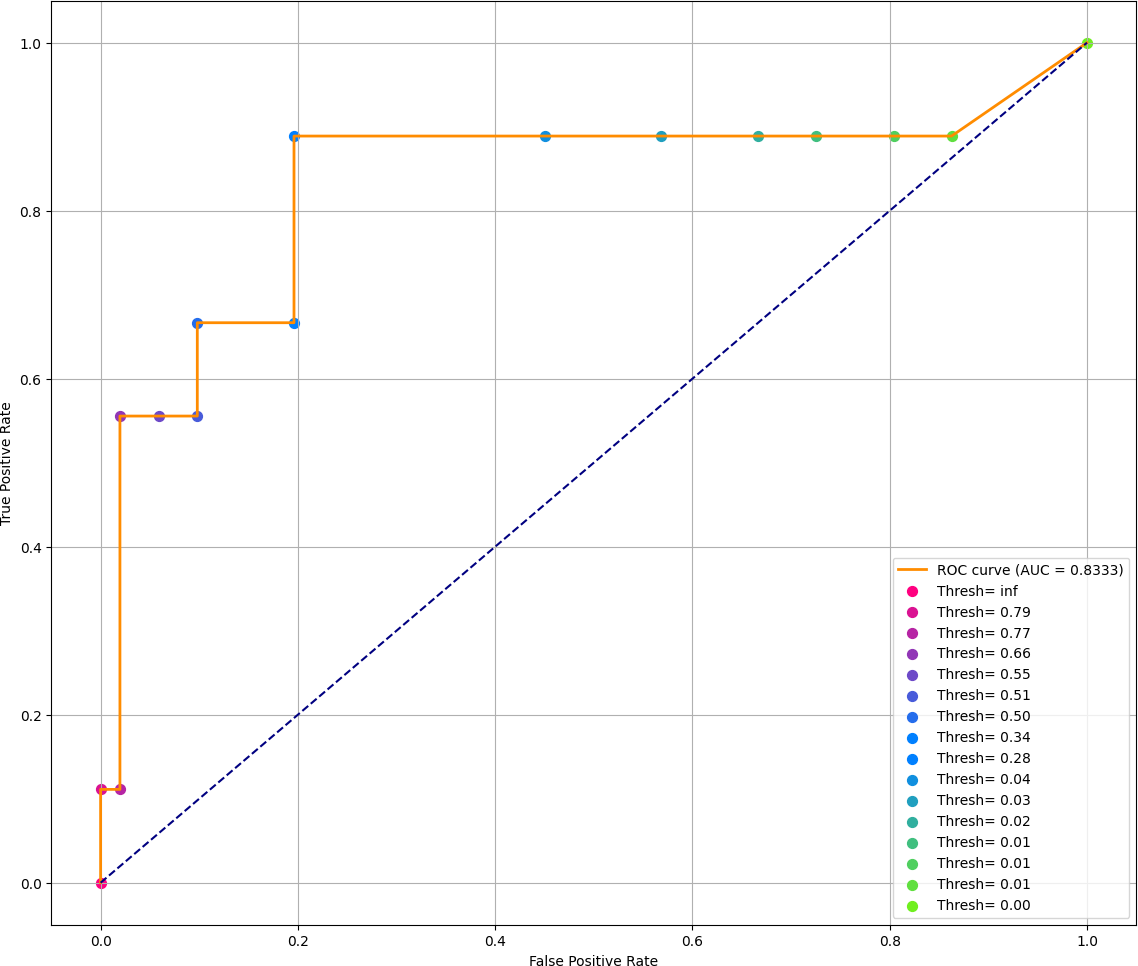
\includegraphics[width=0.9\textwidth]{ROC_AUC_result_best_joint.png}
  \caption{ROC curve of the most frequent joint of the dataset}
  \label{fig:roc_auc_results}
\end{figure}